\chapter{INTRODUCTION}
\label{chap:introduction}

\begin{figure} [tb]
  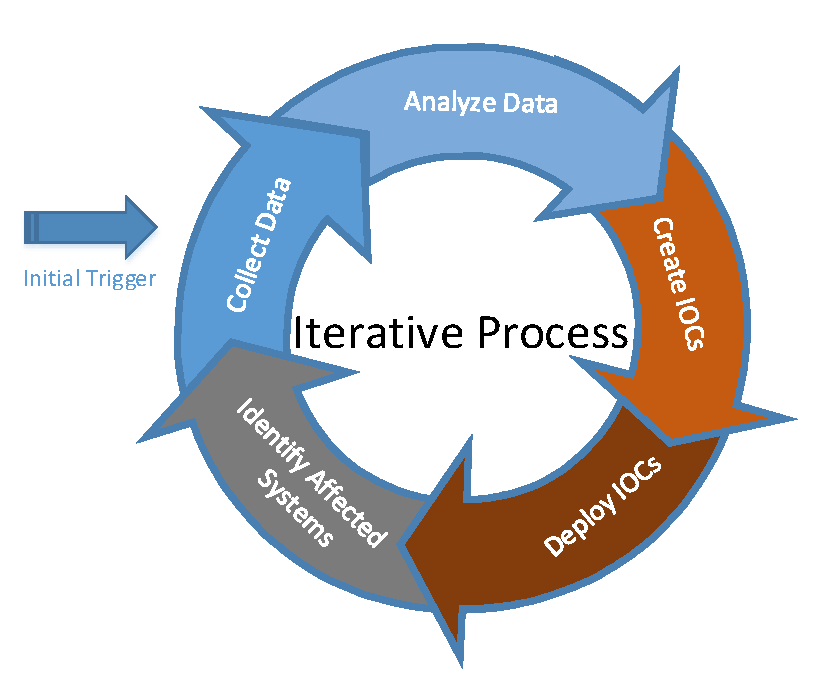
\includegraphics[width=14cm, height=10cm]{lifecycle.pdf}
  \caption [\titlecap{IOC lifecycle}] {IOC Lifecycle. The process starts from the collection of data from internal (e.g., malware analysis reports, network logs, etc.) and external (e.g., security blogs, security white-papers, etc.) sources. Data analysis identifies the IOCs using log analysis, forensics analysis, false positive identification, etc. All IOCs are converted into security formats such as OpenIOC~\cite{openioc}, snort~\cite{snort}, etc., during the IOC creation step. Then, these IOCs are deployed on security tools such as Intrusion Detection Systems (IDS), Host based Intrusion Detection Systems (HIDS), Security Information and Event Management (SIEM), and other investigative systems~\cite{lunt}. During the $5^{th}$ stage, suspected systems are identified. Then, log data and forensic images of suspected systems are provided to the data collection step for the creation of new IOCs. }
  \label{fig:ioc}
\end{figure}

\paragraph{}
According to Verizon's 2016 Data Breach Investigations Report~\cite{verizon}, over 100,000 security incidents were reported in 2016 across 82 countries, which is a 25\% increase over the prior year. Because the number of security threats and breaches is rapidly increasing over time, every organization is attempting to protect their systems and their data. The threat landscape is always progressing, and the information security risk is increasing because of the organization's dependence on computing systems. This constantly shifting and constantly increasing number of threats results in tremendous pressure on organizations to manage threats.
% Adam: I don't understand what the next two sentences are trying to say. Could they be reworded?
Though abundant information is available in the form of unstructured data, it is very difficult and time-consuming to mine meaningful information based on which preemptive measures can be established. This attracts more and more researchers towards Threat Intelligence (TI) as it helps to understand threats using the deluge of data and provides actionable insights.

Threat intelligence (TI) is proof-based knowledge, which includes reasoning, context, mechanism, indicators, implications, and actionable advice, about an existing or evolving cyber-attack that can be used to create preventive measures in advance~\cite{rob}.  Attackers consistently exploit systems and networks to steal sensitive information, to take control of the target system, or for ransom (using ransomware)~\cite{gorman}. TI allows an organization to expand its visibility into the fast-growing threat landscape, can allow early identification of an attack, and successfully prevent the attack. 

Indicators of Compromise (IOCs) are forensic artifacts that are used as signs that a system has been compromised by an attacker or that a system has been infected with a particular piece of malware~\cite{catakoglu}. The intent of accumulating IOCs related to malware or an attack is to be able to state, with a relatively high degree of confidence, whether or not such artifacts are present in a given environment. The goal of TI is to help security professional provide data-backed reasoning of why an artifact is identified as an IOC or not. Concretely, IOCs are composed of some combination of IP addresses, hostnames, filenames, processes, services, Windows registry entries, or hashes~\cite{andress}.

Figure~\ref{fig:ioc} explains the typical life cycle for the use of IOCs in an organization. This life cycle consists of five steps: data collection, data analysis, IOC creation, deployment of IOCs on security infrastructure, and identification of affected systems using deployed IOCs. As a final step, log data of these compromised systems is collected and used for the creation new IOCs, which feeds back into the IOC life cycle in a cyclical way.


Several standards are commonly used to represent IOCs for expressing cyber-threat intelligence information such as: OpenIOC~\cite{openioc}, Structured Threat Information eXpression (STIX)~\cite{stix}, Cyber Observable eXpression (CybOX)~\cite{cybox}, Trusted Automated eXchange of Indicator Information (TAXII)~\cite{taxii}, Snort~\cite{snort}, Suricata~\cite{suricata}, YARA~\cite{yara}, Malware Attribute Enumeration and Characterization (MAEC)~\cite{maec}, and Common Attack Pattern Enumeration and Classification (CAPEC)~\cite{capec}.

\paragraph{} % Importance of IOCs
IOCs can help an organizations' security personnel to attain full automation: Given a set of IOCs for a particular security event, security tools scan through an environment or infrastructure to identify the existence of any IOC on the systems in question. IOCs complement and augment existing solutions, such as Intrusion Detection Systems (IDS) or Security Information and Event Managements (SIEMs), by providing an additional and important set of information that can be used to decide whether a particular artifact being examined is malicious or not. IOCs provide a rapid route to detect new or zero-day attacks for which virus signatures or detection rules have yet to be developed for existing security tools. Thus, timely generation of IOCs is important. Also, IOC formats document a threat in a consistent fashion, thus it becomes easier for organizations to share this threat information. 


\paragraph{} % Limitations
However, effective collection and sharing of threat information is a challenge. Current threat intelligence systems have following limitations: 
\begin{itemize}
 \item[$\bullet$ ] Threat data received from different sources, such as malware reports, APT white-papers, etc., is examined and interpreted
by security analysts \emph{manually}, a procedure that is timely and error-prone, which limits the practical usefulness of this
data in an organizations' security infrastructure. 
  \item[$\bullet$ ] Most of the traditional approaches consider either one or two data sources for the generation of Indicators of Compromises
(IOCs) and miss valuable IOCs from alternative data sources, such as blog articles about recent attacks.
  \item[$\bullet$ ] Current state-of-the-art lacks support of diverse IOC formats (e.g., STIX, OpenIOC, or snort) which further reduces the effectiveness of these tools. 
\item[$\bullet$ ] Most importantly, many TI tools generate IOCs directly using regular expressions and white-listings from security literature or blog articles~\cite{otx} without understanding the contextual meaning of those IOCs from the data sources which allows the tools to include lot of false positives during the process of IOCs creation.
\end{itemize}

%iGen is tackling all these limitation by intelligently collecting and exchanging the information in the form of IOCs (e.g. virus signatures, IPs, domains, MD5 hashes etc.). After the collection, iGen automatically transforms these IOCs into different threat information sharing standards such as STIX , OpenIOC , and Snort rules etc. and fed into different defense mechanisms (e.g. Intrusion Detection Systems (IDS) etc). Biggest challenge in the field of TI is to intelligently gather such information from large amount of data and timely deploy it on defense mechanisms.

\paragraph{} % iGen
In this project we present iGen, which is a system that tackles all of these limitation by intelligently collecting threat information from publicly available security resources and sharing the threat information in the form of IOCs (e.g., virus signatures, IPs, domains, or MD5 hashes). iGen automates the entire process of collecting publicly available data (data collection) to IOC generation. iGen supports a flexible system to collect data from diverse data sources. Currently, iGen collects data from 20 security blogs, an APT reports database~\cite{apt}, and a malware analysis system. The flexible nature of the system means that new data sources can be easily added. Note that the input to iGen is in unstructured English text, therefore iGen must understand the semantics of the sentences present in the input data to categorize IOC-alike strings into IOC or non-IOCs. Also, we added a practical improvement to iGen that allows transforming these IOCs into various threat information sharing standards.

% Adam: This is way too much detail for the intro
First module in iGen is data acquisition module which collects key observations from the data sources like APT reports, malware analysis reports and blog articles. This module collects these reports in real-time and keep iGen updated with new IOCs from recent malware and APTs. In parallel, malware analysis system looks for new malware on web and generate malware analysis report for those samples.   All the different kinds of reports accumulated from different data sources are then presented to machine learning based IOC extractor. IOC extractor module decides the parsing strategy based on the type of report. Since, malware analysis reports are based on real malware and available in machine readable format (e.g. JSON file). In this case, IOC extraction was done using a parser which accrue IOCs based on the JSON schema. But security reports or blog articles are relatively complex which tend to describe IOCs in intricate manner in English text using some context terms like ``download'', ``malware'' etc. Google's tensorflow~\cite{abadi} based Convolutional Neural Netowrk~\cite{krizhevsky} model was used to classification all the sentences in these reports into IOC or non-IOC sentences~\cite{bengio,yih,mikolov,collobert}. Once sentence classification is done, next step is to identify IOCs intelligently. More explicitly, after classifying the sentence in the article into IOC and non-IOC sentences. iGen utilizes a set of regular expressions (regex) to locate IOC tokens (e.g., IP, hostname, domain, md5 etc.) within the sentence. Then, iGen extract these IOC tokens and convert them to machine-readable formats (IOC formats) which can be used directly by security tools.

Simple extraction of IOCs from publicly available security resources is straightforward: regular expressions can extract MD5s, URLs, filenames, filepaths, etc. However, this na\"{\i}ve approach will result in a significant amount of false positives: these security resources will include MD5s, URLs, and filenames that are \emph{relevant to the security incident but are not malicious, and thus not an IOC}. Therefore, we need an approach that can automatically filter these potential IOCs \emph{based on the context}.
While prior work has shown that filtering potential IOCs can be done with manual creation of features~\cite{liao}, iGen leverages a deep-learning Convolutional Neural Network, which selects features automatically. This enables iGen to be more effective and to use diverse data sets. 

\paragraph{Structure of document} % short describe the sections 
This thesis document is grouped into the following sections:
\begin{itemize}
	\item Chapter 2 discusses the basics of Threat Intelligence (TI) as well as different formats for sharing threat intelligence. This chapter also describes the Convolutional Neural Networks (CNN) which is a core of iGen system. 
	\item Chapter 3 discusses the data collection from different sources.
	\item Chapter 4 discusses the System design, the architecture, and the components of iGen system.
	\item Chapter 5 discusses the implementation details of iGen system.
	\item Chapter 6 presents our findings and comparative analysis of the results.
	\item Chapter 7 continues the discussion of the results; the lessons learned, limitations, and improvements that are possible on current iGen system.
	\item Chapter 8 explores related work in the area.
	\item Chapter 9 concludes this thesis, with ideas to develop the research in this area.
\end{itemize}

\paragraph{} % Contribution
The main contributions of this paper are the following:
\begin{itemize}
 \item[$\bullet$ ] We present the design of a novel system for intelligently generating IOCs, with high confidence, from different data sources using Convolutional Neural Networks (CNNs) (Section 3). 
  \item[$\bullet$ ] A prototype implementation of our design in a tool called iGen (Section 4).
  \item[$\bullet$ ] An evaluation of iGen with other state-of-the-art methods. iGen identified around 400,000 IOCs with a precision and recall of 95\% and 99\% respectively (Section 5). 
\end{itemize}
